\RequirePackage{luatex85}
\documentclass[a4paper,sfsidenotes,twoside,justified]{tufte-book-custom}
% \usepackage{showframe}

\hypersetup{colorlinks}

\title[On Homomorphism Problems]{ Homomorphism\\ Problems: from Minimization of Graph Databases Queries to the Frontier of Decidability in Automatic Structures}
\author[The Tufte-LaTeX Developers]{The Tufte-LaTeX\ Developers}
\publisher{Publisher of This Book}

\usepackage{xcolor}

% ---
% German color palette
% ---

% https://flatuicolors.com/palette/de
\definecolor{Desire}{HTML}{eb3b5a} % red
\definecolor{Boyzone}{HTML}{2d98da} % blue
\definecolor{Royal Blue}{HTML}{3867d6} % darker blue
\definecolor{NYC Taxi}{HTML}{f7b731} % yellow
\definecolor{Algal Fuel}{HTML}{20bf6b} % green
\definecolor{Innuendo}{HTML}{a5b1c2} % grey
\definecolor{Twinkle Blue}{HTML}{d1d8e0} % light grey
\definecolor{Gloomy Purple}{HTML}{8854d0} % dark purple

% ---
% Synonyms
% ---

\colorlet{cBlue}{Royal Blue}
\colorlet{cYellow}{NYC Taxi}
\colorlet{cGreen}{Algal Fuel}
\colorlet{cRed}{Desire}
\colorlet{cGrey}{Innuendo}
\colorlet{cLightGrey}{Twinkle Blue}
\colorlet{cPurple}{Gloomy Purple}

% ---
% Colors for knowledge
% ---

\colorlet{KlDefn}{cRed!60!black} 
\colorlet{KlLink}{cBlue!40!black}
\colorlet{KlWarning}{cYellow!60!black}

\colorlet{maincolor}{Boyzone}
\usepackage{polyglossia}
\setmainlanguage{english}

\usepackage[protrusion=true,expansion,babel]{microtype}
\usepackage{booktabs}
\usepackage{graphicx}
\usepackage{lipsum}
\usepackage{stmaryrd}
\usepackage{multicol,multirow}
\usepackage{ifthen}
% \usepackage{subcaption}
\usepackage{epigraph}
\usepackage{proof}
\usepackage[export]{adjustbox} % valign for includegraphics
\usepackage{stackengine}
\usepackage{etoolbox} % \renewrobustcmd

\usepackage{appendix,chngcntr} % appendix after each chapter
% see https://tex.stackexchange.com/questions/120716/appendix-after-each-chapter
% Start of subappendices environment
\AtBeginEnvironment{subappendices}{%
\section*{Appendices}
% \addcontentsline{toc}{chapter}{Appendices}
\counterwithin{figure}{section}
\counterwithin{table}{section}
}
% End of subappendices environment
\AtEndEnvironment{subappendices}{%
\counterwithout{figure}{section}
\counterwithout{table}{section}
}

\usepackage{listings}
\lstdefinestyle{mystyle}{
    backgroundcolor=\color{cLightGrey!30!white},   
    % commentstyle=\color{codegreen},
    keywordstyle=\color{maincolor},
    % numberstyle=\numberstyle,
    stringstyle=\color{cBlue},
    basicstyle=\footnotesize\sffamily,
    % breakatwhitespace=false,
    % breaklines=true,
    % captionpos=b,
    keepspaces=true,
    % numbers=left,
    % numbersep=10pt,
    showspaces=false,
    showstringspaces=false,
    showtabs=false,
	tabsize=4,
	framesep=8pt,
	frame=tblr,
	framerule=0pt
}
\lstset{style=mystyle}

\usepackage[most]{tcolorbox}
\usepackage{bbding} % \HandRight
% Lettrines
% \usepackage{lettrine}
% \newfontface\gleaf{GothicLeaf-VEay}
% \renewcommand{\LettrineFontHook}{\gleaf}
% \setcounter{DefaultLines}{3}
\usepackage[capitalise]{cleveref}
\usepackage[xcolor, hyperref, notion, quotation, makeidx, composition]{knowledge}
\usepackage{mathcommand}
\knowledgeconfigure{quotation, protect quotation={tikzcd}}
\knowledgeconfigure{diagnose line=true, diagnose bar=true}

% \def\notionKnowledgeIndexIntroStyle#1{\textcolor{maincolor}{\textbf{#1}}}

\IfKnowledgePaperModeTF{
}{
    % If we are NOT in paper mode (i.e. in composition mode or electronic mode)
    \knowledgestyle{intro notion}{color={KlDefn}, emphasize, index style=textbf}
    \knowledgestyle{notion}{color={KlLink}}
    \hypersetup{
        colorlinks=true,
        breaklinks=true,
        linkcolor={KlLink}, % Links to sections, pages, etc.
        citecolor={KlCite}, % Links to bibliography
        filecolor={KlLink}, % Links to local file
        urlcolor={KlUrl}, % Links for URLs
    }
    \IfKnowledgeElectronicModeTF{
        %
    }{
        % If we are in composition mode, highlight unknown stuff (in yellow) and display the anchor point.
        \knowledgeconfigure{anchor point color={KlDefn}, anchor point shape=corner}
        \knowledgestyle{intro unknown}{color={KlWarning}, emphasize}
        \knowledgestyle{intro unknown cont}{color={KlWarning}, emphasize}
        \knowledgestyle{kl unknown}{color={KlWarning}}
        \knowledgestyle{kl unknown cont}{color={KlWarning}}
    }
}

% ---
% Correctly handling \mathop/\mathrel with \knowledgenewrobuscmd
% ---
% \ExplSyntaxOn
% \RenewDocumentCommand\withkl{mm}{
% \int_gincr:N\knowledge_inner_modifier_count_int
% \cs_gset:cpx
% {\knowledge_inner_command:}
% {\exp_not:N\cs_gset:Npn
% \exp_not:c{\knowledge_inner_command:}
% {\knowledge_inner_modifer_re_tl\knowledge_kl_modifiers_tl\exp_not:n{#1}}
% \knowledge_kl_modifiers_tl\exp_not:n{#1}}
% \knowledge_kl_modifiers_reset:
% #2
% \int_gdecr:N\knowledge_inner_modifier_count_int
% }
% \ExplSyntaxOff

% \def\notionKnowledgeIndexIntroStyle#1{\textcolor{maincolor}{#1}}
\newrobustcmd{\fancyand}{{\setmainfont{Tex Gyre Pagella}\textit{\&}}}

\newrobustcmd\decisionproblem[3]{
	\begin{center}\AP
	\fbox{\begin{tabular}{rl}
	\multicolumn{2}{l}{#1} \\\midrule
	{\emph{Input}}: & \parbox[t]{.73\linewidth}{#2} \\   
	{\emph{Question}}: & \parbox[t]{.73\linewidth}{#3}
	\end{tabular}} 
	\end{center}
}

\usepackage{adforn}
\newrobustcmd{\proofcase}[1]{\adforn{39}~\emph{#1}~}
\newrobustcmd\?{\symbf}
\newrobustcmd\+{\symcal}
\newrobustcmd\•{\symcal}
\newrobustcmd\B{\symbb}

\newrobustcmd\card[1]{|1|}
\newcommand{\set}[1]{\{#1\}}
\newcommand{\tup}[1]{\langle#1\rangle}

\knowledgenewrobustcmd\pset[1]{\cmdkl{\symfrak{P}(#1)}} % powerset
\knowledgenewrobustcmd\psetp[1]{\cmdkl{\symfrak{P}_+(#1)}} % strict powerset

\newcommand{\dcup}{\sqcup} % disjoint union of sets
\newcommand{\bigdcup}{\bigsqcup} % disjoint union of sets

\knowledgenewrobustcmd\id[1][]{\cmdkl{\mathrm{id}_{#1}}} % identity function

\newrobustcmd\N{\symbb{N}} % natural numbers
\newrobustcmd\Np{\N_{>0}} % strictly positive nat. numbers
\newrobustcmd\Z{\symbb{Z}}
\newrobustcmd\ZnZ[1]{\symbb{Z}/#1\symbb{Z}}

\newrobustcmd\defeq{\mathrel{\hat{=}}} % equality by definition
\newrobustcmd\pto{\rightharpoonup} % partial function
\knowledgenewrobustcmd{\equivclass}[2][]{[#2]^{#1}} % equivalence class

\knowledgenewrobustcmd\restr[2]{{% function restriction
  #1 \cmdkl{\raisebox{-.1em}{\(\vert\)}{}_{#2}}
}}

% ---
% Basic
% ---

\knowledgenewrobustcmd{\transition}[1]{\mathrel{\cmdkl{\smashxrightarrow{\ensuremath{#1}}}}}

\knowledgenewrobustcmd{\semFO}[2]{\cmdkl{\lBrack} #1 \cmdkl{\rBrack^{#2}}} % semantics of FO
\disablecommand{\models}
\suggestcommand\models{\FOmodels}
\knowledgenewrobustcmd\FOmodels{\mathrel{\cmdkl{\LaTeXmodels}}} % models relation


\newrobustcmd\Acc{\textrm{Acc}}
\newrobustcmd\Bcc{\textrm{Bcc}}
\knowledgenewrobustcmd\semTM[1]{\cmdkl{\lBrack}#1\cmdkl{\rBrack}} % semantics of Turing machine
\knowledgenewrobustcmd\statesTM[1]{\cmdkl{Q^{#1}}} % states of Turing machine

% ---
% Relational structures
% ---
\knowledgenewrobustcmd{\neighbourhood}[4]{\cmdkl{\+N_{\!#2}^{\smash{#3,#4}}(#1)}}
\knowledgenewrobustcmd{\ball}[3]{\cmdkl{\+B}_{#1}^{#3}(#2)}
\knowledgenewrobustcmd{\IncidenceGraph}[1]{\cmdkl{\mathrm{Inc}(#1)}}

% ---
% Hom & core
% ---
\knowledgenewrobustcmd{\homto}{\mathrel{\cmdkl{\smashxrightarrow{hom}}}}
\newrobustcmd{\cohomto}{\mathrel{\kl[\homto]{\smashxleftarrow{hom}}}}
\RequirePackage{centernot}
\newrobustcmd{\nothomto}{\mathrel{\kl[\homto]{\centernot{\smashxrightarrow{hom}}}}}
\newrobustcmd{\notcohomto}{\mathrel{\kl[\homto]{\centernot{\smashxleftarrow{hom}}}}}

\knowledgenewrobustcmd\core[1]{\cmdkl{\check{{#1}}}}

% ---
% Constructions on structures
% --- 
\knowledgenewrobustcmd\prodstruct{\mathbin{\cmdkl{\times}}}
\knowledgenewrobustcmd\powstruct[2]{\cmdkl{#1^{#2}}}
\knowledgenewrobustcmd\iterstruct[2]{\cmdkl{#1^{#2}}}

\input{kl/abbreviations.kl}
\input{kl/complexity.kl}
\input{kl/misc.kl}

\setcounter{secnumdepth}{3}

\begin{document}

\frontmatter
\newgeometry{hmargin=2.5cm, top=4.5cm, bottom=3cm}
\begin{titlepage}
\begin{center}
  \Huge\scshape%
  Homomorphism Problems
  \LARGE\\
  in Graph Databases\\
  and Automatic Structures\\
  % \vspace{5cm}
  % \makebox[0pt]{{%
  %   \fontsize{50}{0}\selectfont\color{black!11}%
  %   $\gamma \equiv^{?} \delta$%
  % }}{}\\
  \vfill
  \normalfont\LARGE{} \textsc{Rémi Morvan}\\[1em]
  \Large\scshape
  Ph.D. thesis in Computer Science\\
  \textcolor{maincolor}{LaBRI, Université de Bordeaux}\\
  \normalfont\Large\scshape To be defended on 3rd July 2025
\end{center}
\end{titlepage}
\restoregeometry
\newpage
\thispagestyle{empty}
~
\newpage
\thispagestyle{empty}
% \setlength{\parskip}{\baselineskip}
\begin{fullwidth}
	\setlength{\parindent}{0pt}
	~\vfill
	\begin{center}
		\normalfont\Large\scshape Composition of the jury:\\[1.5em]
		\normalfont
		\begin{tabular}{r@{\hskip 1em}l@{\hskip 1em}l}
		  Mikołaj Bojańczyk & \textsc{\small Uniwersytet Warszawski} & \emph{reviewer {\small\fancyand}~examiner}\\
		  Wim Martens & \textsc{\small Universität Bayreuth} & \emph{\hphantom{revi}``} \\[.5em]
		  Antoine Amarilli & \textsc{\small Inria, Lille} & \emph{examiner}\\
		  Balder ten Cate & \textsc{\small Universiteit van Amsterdam} & \emph{\hphantom{revi}``}\\
		  Bartek Klin & \textsc{\small University of Oxford} & \emph{\hphantom{revi}``}\\
		  Anca Muscholl & \textsc{\small Université de Bordeaux} & \emph{\hphantom{revi}``}\\
		  Sophie Tison & \textsc{\small Université de Lille} & \emph{\hphantom{revi}``}\\[.5em]
		  Diego Figueira & \textsc{\small CNRS, Bordeaux} & \emph{supervisor}\\
		  Nathanaël Fijalkow & \textsc{\small CNRS, Bordeaux} & \emph{co-supervisor}
		  % Sophie Tisson
		\end{tabular}
	\end{center}

	\vfill

	\par\textsc{Licensed under "CC BY 4.0".}
	\par\textit{Version of \today.}
\end{fullwidth}
% r.5 contents
{ % env necessary for the parskip not to leak in the rest of the doc.
	\setlength{\parskip}{0em}
	% \addcontentsline{toc}{chapter}{Contents}
	\setcounter{tocdepth}{1}
	\tableofcontents
}
% \listoffigures
% \listoftables

% % r.7 dedication
% \cleardoublepage
% ~\vfill
% \begin{doublespace}
% \noindent\fontsize{18}{22}\selectfont\itshape
% \nohyphenation
% Dedicated to those who appreciate \LaTeX{} 
% and the work of \mbox{Edward R.~Tufte} 
% and \mbox{Donald E.~Knuth}.
% \end{doublespace}
% \vfill
% \vfill

\mainmatter
\chapter{Ideas/Todos}

\begin{itemize}
	\item Change definition of CQ/CRPQ to have vertices. This allows for better duality,
		and also better statement for the Semantical Structure Theorem (in some prop we get
		``foo is an edge contraction of bla'' instead of ``is a minor of'').
		Update the definition of `one-way internal path' to allow for $n=0$.
	\item Extend the notion of `strong minimality` using the axioms used in the lower bound (`str-onto`): call such canonical databases / extensions `structurally minimal'.
	Prove or disprove the following result: ``a "CRPQ" has "one-way semantic tree-width" at least $k$ "iff" it has an expansion that is structurally minimal and whose core has tree-width at least $k$''. In general: what about minor-closed classes?
	Extend Grohe's Theorem to CRPQs (or maybe to a subclass of CRPQs, "eg" those whose
	structurally minimal canonical databases characterize membership to minor-closed classes).
\end{itemize}

\chapter{Introduction}

\part{Querying Graph Databases}

\chapter{Preliminaries on Graph Databases}

\section{Elementary Notations}

\subsection{Blabla}

% \begin{figure}
% 	\centering
% 	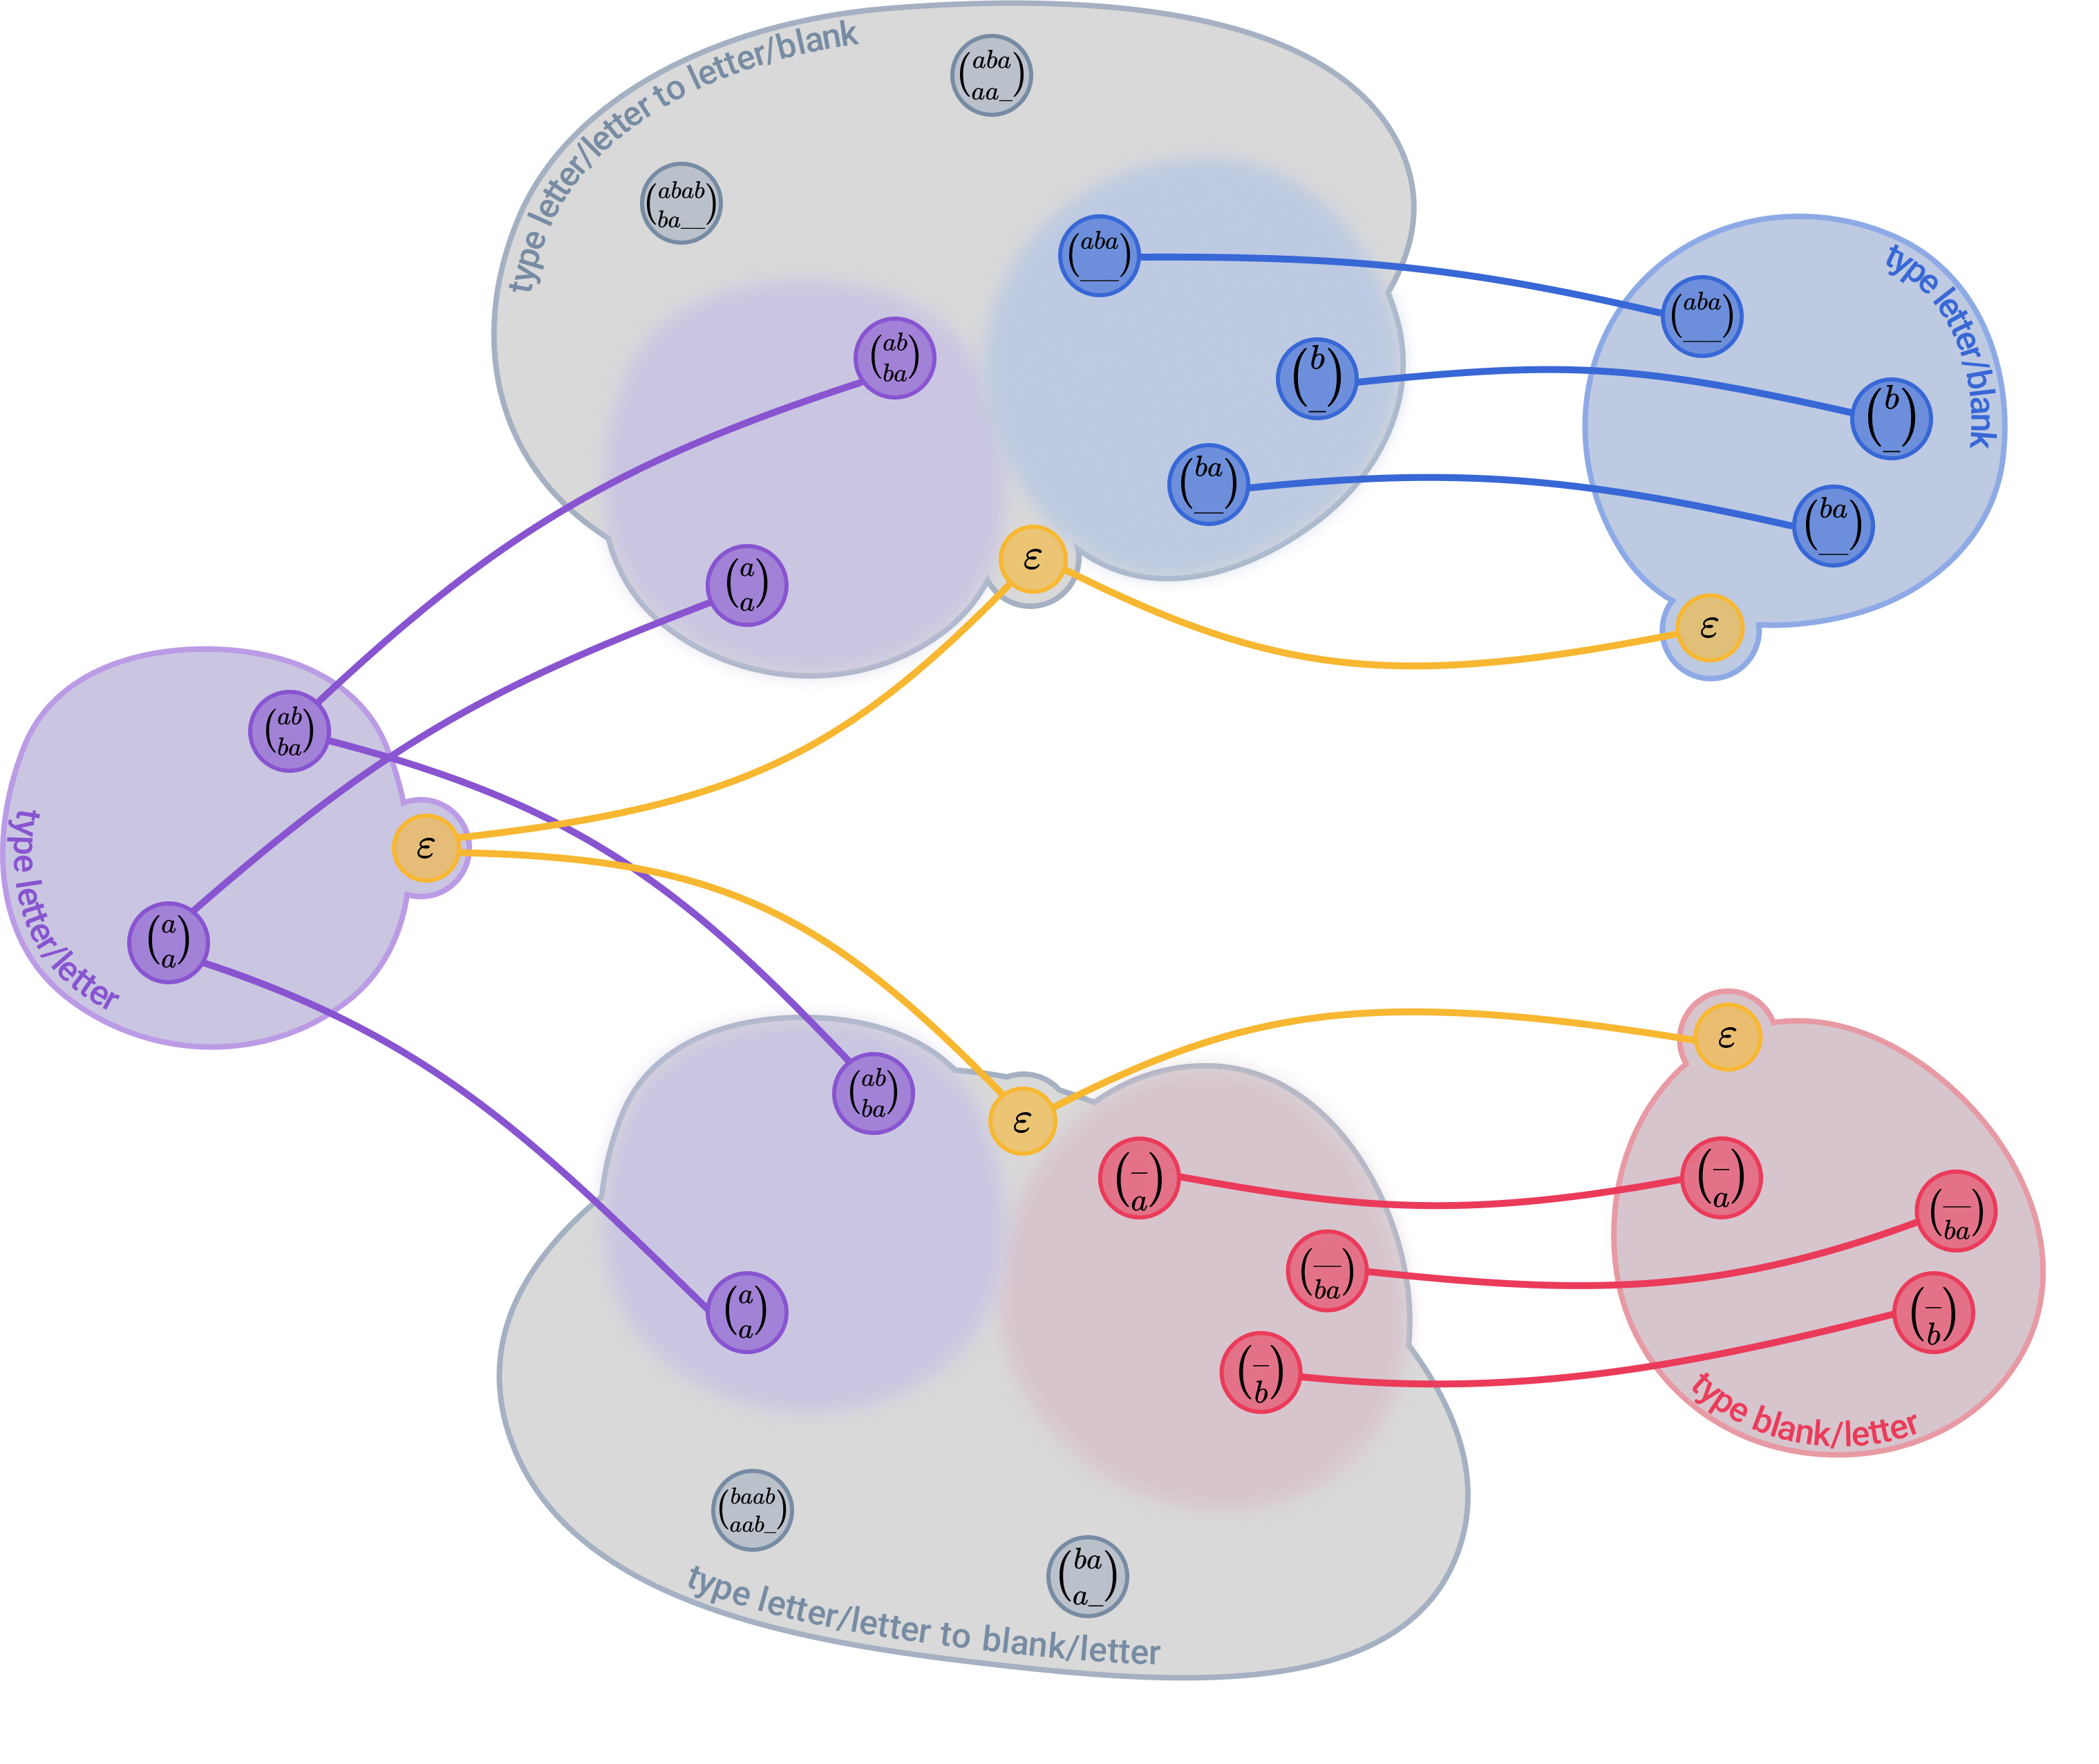
\includegraphics[width=\linewidth]{fig/free_algebras.png}
% 	\caption{My super nice caption.}
% \end{figure}

\begin{table}
	\centering
	\begin{tabular}{cc}
		\toprule
		a & b \\ \midrule
		0 & 1 \\
		1 & 0 \\ \bottomrule
	\end{tabular}
	\caption{My super nice caption.}
\end{table}

Hello this is a citation\cite{Bringhurst2005}.
Hello Q\sidenote{Qy first sidenote!} world\sidenote{Another side note}.
\[\forall x \in \gamma,\, \exists y\in \delta, \delta \to \gamma\]
\[L \subseteq \Sigma^*\]
\[0 \in \mathbb{N}\]
\[\mathcal{AbcDefGhiJkl}\]

\lipsum[1-2]

\begin{figure}[htb]
	\centering
	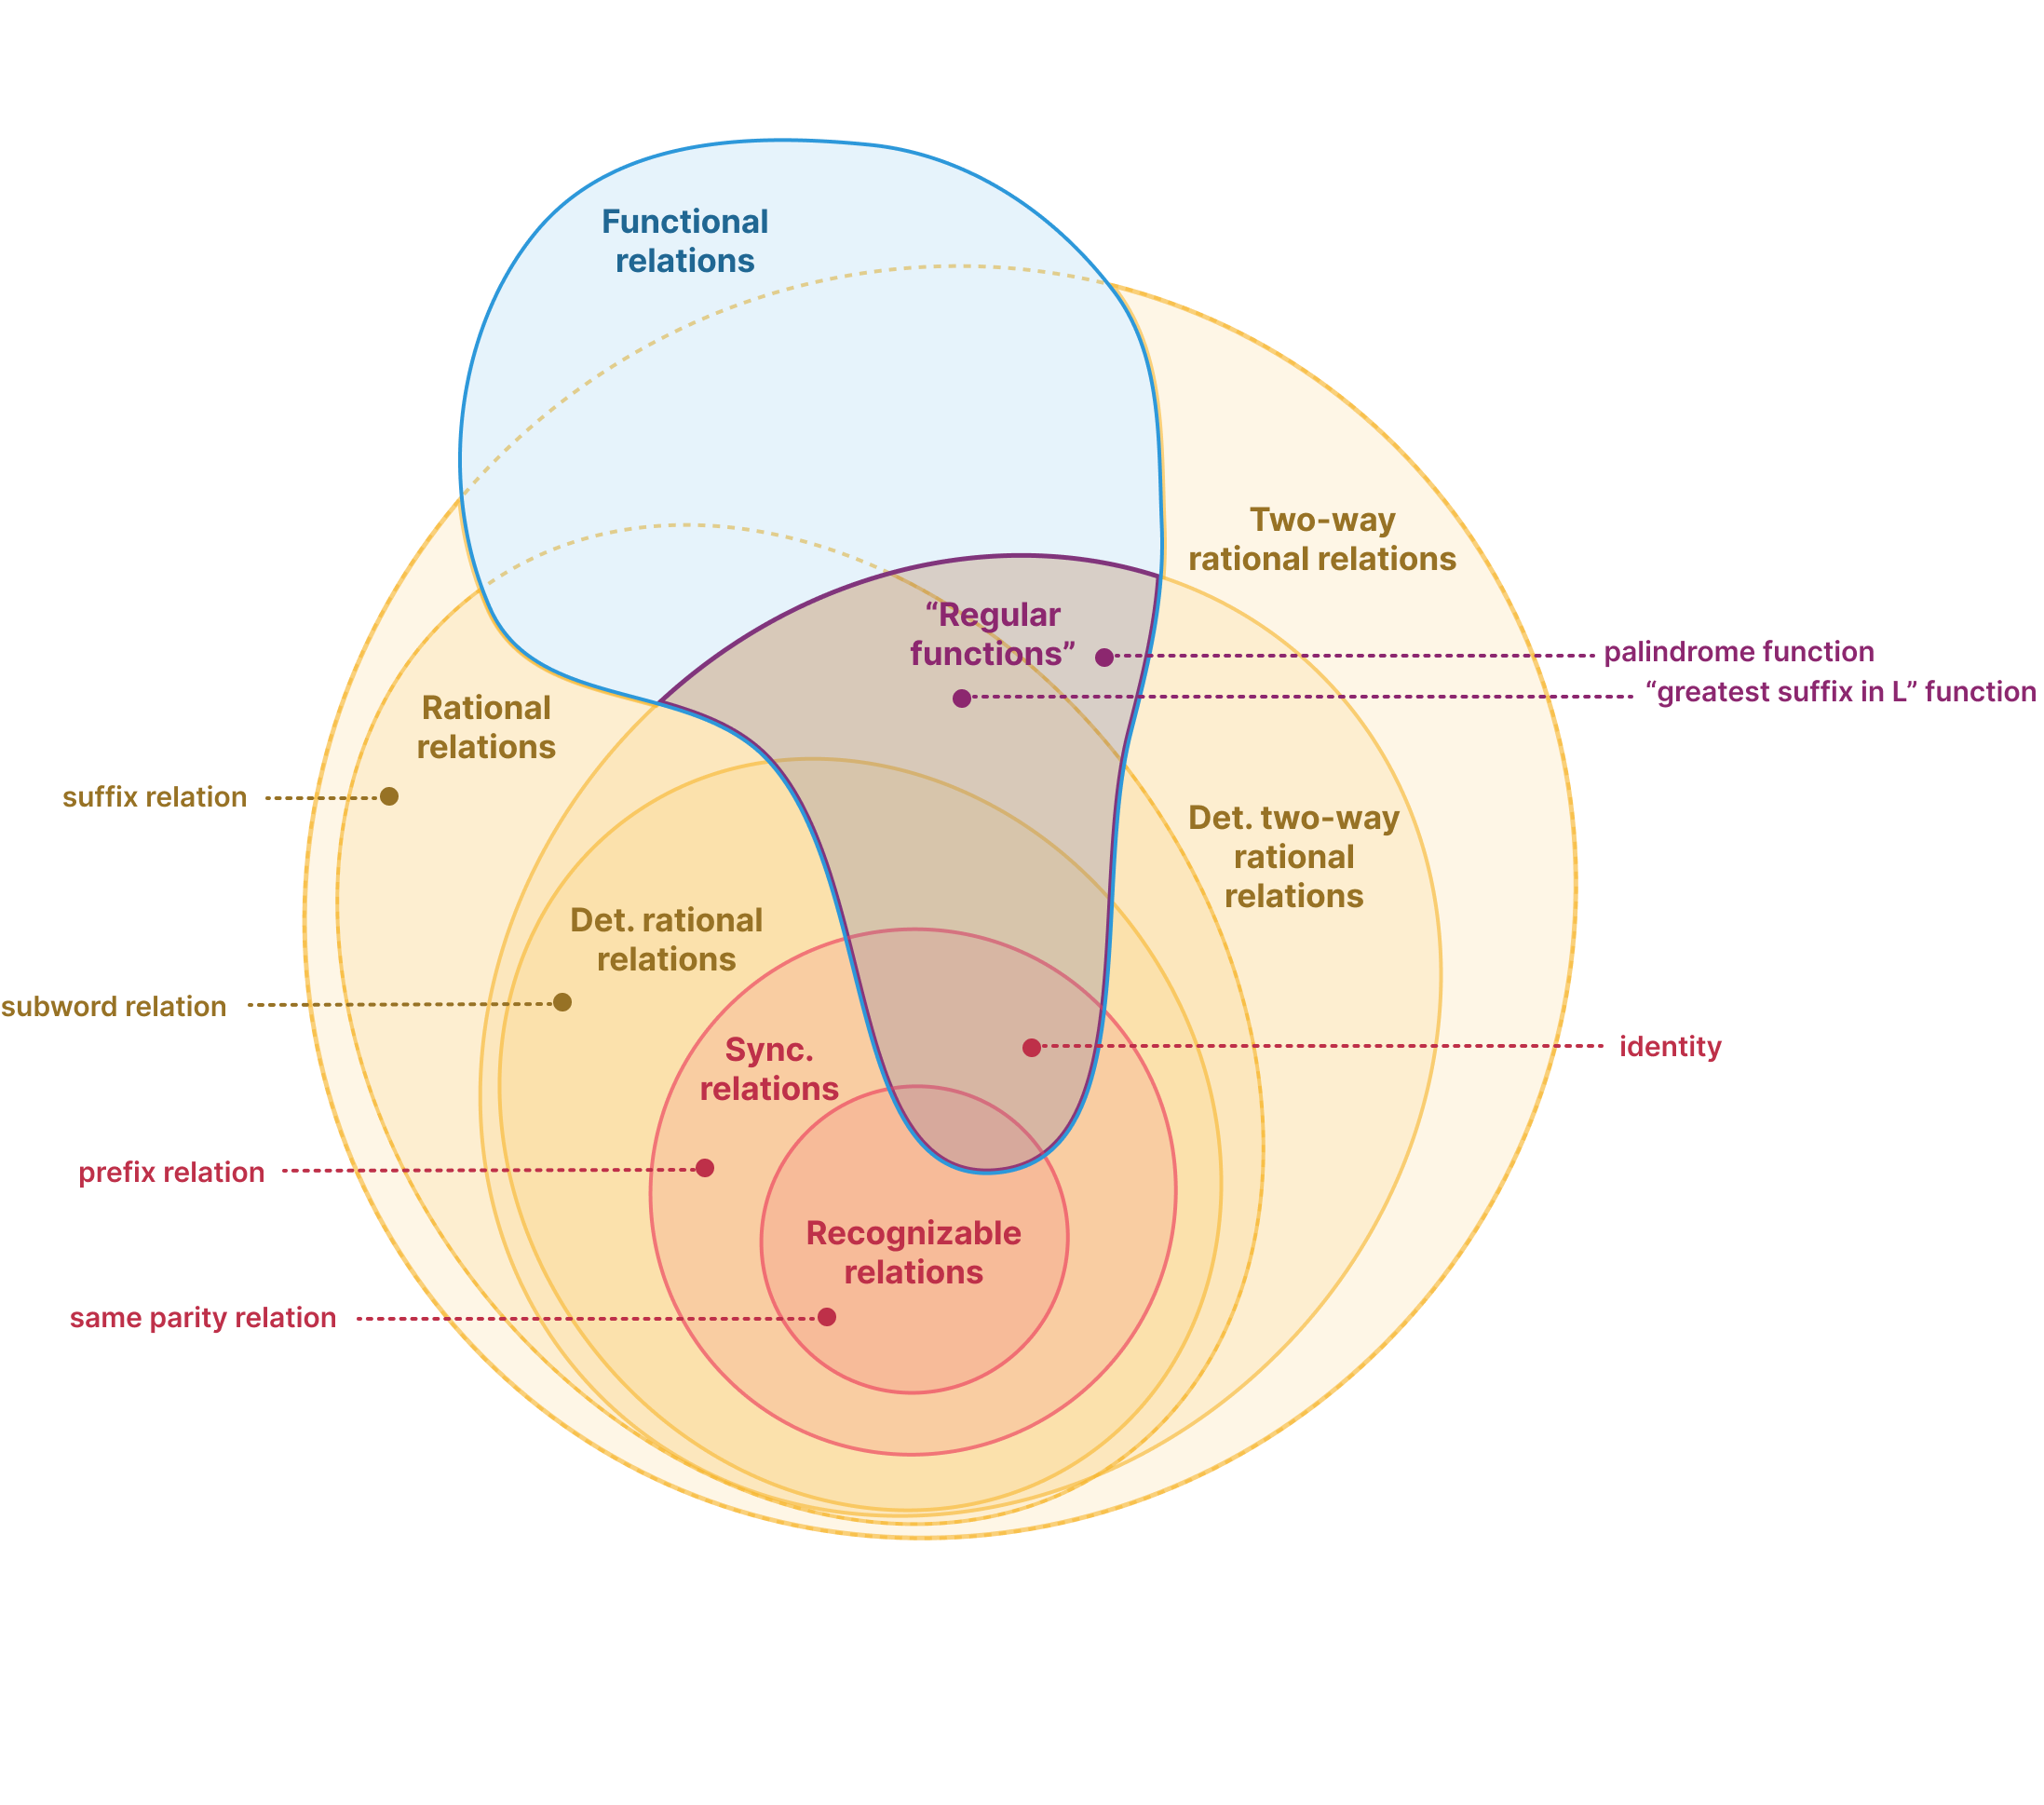
\includegraphics[width=\linewidth]{fig/landscape.png}
	\caption{The landscape of rationality.}
\end{figure}

\lipsum[3-10]

\chapter[Evaluation and Containment of Conjunctive Regular Path Queries]{Evaluation and Containment\\ of Conjunctive Regular Path Queries}

\chapter{Minimization of Conjunctive Regular Path Queries}

\chapter[{Semantic Tree-Width and Path-Width of Conjunctive Regular Path Queries}]{Semantic Tree-Width and Path-Width\\of Conjunctive Regular Path Queries}

\chapter{Synthesis of Conjunctive Regular Path Queries}

\chapter{Conclusion \& Open Problems}

\part[The Frontier of Decidability in Automatic Structures]{The Frontier of Decidability\\in Automatic Structures}

\chapter{Preliminaries on Automatic Structures}

\chapter{A Dichotomy Theorem for Automatic Structures}

\chapter{The Algebras for Automatic Relations and Beyond:\\the Relative Membership Problem for Pseudovarieties of Regular Languages}

\chapter{Conclusion \fancyand~Open Problems}


\backmatter

\bibliography{sample-handout}
\bibliographystyle{plainnat}

\end{document}

